% !TeX spellcheck = en_US
\documentclass[a4paper,12pt]{article}
\usepackage[utf8x]{inputenc}
\usepackage{wrapfig}
\usepackage{graphicx}
\usepackage{float}
\usepackage{listings}
\usepackage{amsmath}
\usepackage{caption}
\usepackage{subcaption}
\usepackage[usenames,dvipsnames,svgnames,table]{xcolor}
\usepackage{datetime}
\usepackage{fancyhdr}
\pagestyle{fancy}

% Title Page
\title{AST3310 Project 1}
\author{Andreas Ellewsen}

\fancyhead[L]{Andreas Ellewsen}
%\fancyhead[C]{Modeling the solar core}
\fancyhead[R]{Spring 2015}

\begin{document}

\maketitle
\tableofcontents
\newpage
\section{Project}
The project involves modeling the central parts of the sun by
writing a computer program to solve the governing equations. The project
involves information contained in Chaps.1-5.

The main point of the project is to solve five equations.
These five equations govern the internal structure of the radiate core of the sun.
By doing so one hopes to make a model of the core of the sun, where the radius, and the luminosity of the star goes to zero, when reducing the mass to zero.
To do this there will be done a series of tests along the way so that one in the end will reach this goal.

\section{Assumptions}
It is assumed that the gas behaves as an ideal gas, and thus obeys the equation of state for an ideal gas.
It is also assumed that all elements are fully ionized.
Only the PPI and PPII chains of the fusion process are included.
And only the evolution of Hydrogen and Helium 4 is calculated.
The only constraint set for the other elements is that the destruction rate can not exceed the production rate of them.

\section{Calculations}
A number of calculations had to be done to complete this assignment.
The first thing I needed to know was the evolution equations for Hydrogen and Helium 4. 
Remember that we simplfied the problem to only evolve these two elements.
The one for Hydrogen can be copied straight from the lecture notes, and when excluding all terms not from the PPI and PPII chain it is
\begin{equation}
\frac{\partial n_p}{\partial t} = \lambda_{pp}n_p^2 - \lambda_{pd} n_pn_{^2_1D} + \lambda_{33} n_{^3_2He}^2 - \lambda_{17}' n_p n_{^7_1Li} 
\end{equation}
and by the same logic, the equation as the first one was found, I found for Helium 4
\begin{equation}
\frac{\partial n_{^4_2He}}{\partial t} = -\lambda_{34}n_{^3_2He}n_{^4_2He} + 2\lambda_{17}' n_p n_{^7_3Li} + \frac{1}{2}\lambda_{33} n_{^3_2He}^2.
\end{equation}

I also need to set restrictions for the reaction rates, so that I don't use elements in reactions faster than they are produced.
Since $r_{33}$ need 2$r_{pp}$ to happen before it, and $r_{34}$ need 1$r_{pp}$ to happen before it, the restriction is set to be
\begin{equation}
 \frac{2}{3}r_{33} + \frac{1}{3}r_{34} \le r_{pp}.
\end{equation}
and with the same logic
\begin{equation}
r_{7e} \le r_{34}
\end{equation}
\begin{equation}
r_{71} \le r_{7e}
\end{equation}
Note that the PPI chain usually happens about 69\% of the time and PPII about 31\%. With the method chosen here, this is not accounted for. By doing it this way the PPI chain only gets 67\%, while PPII gets 31\%. 
Finally, since I want to find the full energy production per units mass $\epsilon = \sum Q_{ik} r_{ik}$, we find the Q values for the different reactions in the chains.
\begin{equation}
\begin{aligned}
Q_{pp}  &= (0.15+1.02) \textrm{ MeV}\\
Q_{dp}  &= 5.49 \textrm{ MeV}\\
Q_{33}  &= 12.86 \textrm{ MeV}\\
Q_{34}  &= 1.59 \textrm{ MeV}\\
Q_{73}  &= 0.05 \textrm{ MeV}\\
Q_{71}  &= 17.35 \textrm{ MeV}\\
\end{aligned}
\end{equation}
This takes care of the energy production.

Next we use the assumption that the gas behaves as an ideal gas, which has equation of state
\begin{equation}
\begin{aligned}
P_G V &= NkT\\
P_G   &= \frac{\rho kT}{\mu m_u}
\end{aligned}
\end{equation}
where $\mu$ is the average mass of the particles in the gas, and $m_u$ is the atomic mass unit.
To find this we need to know what $\mu$ is, and to do that we need to find the total number of particles
\begin{equation*}
\begin{aligned}
n_{tot} &= n_H + n_{He} +n_{Be} + n_{Li} + n_{rest}+ n_e\\
n_{tot} &= n_H + n_{He} +n_{Be} + n_{Li} + n_{rest}+ n_H\\
        & + 2\times3n_{He} + 4n_{Be} + 3n_{Li} + 8n_{rest}\\
n_{tot} &= 2n_H + 7n_{He} + 5n_{Be} + 4n_{Li}+ 9n_{rest}\\
n_{tot} &= 2\frac{X\rho}{m_u} + 7\frac{Y\rho}{4m_u} + 5\frac{Z_{Be}\rho}{7m_u} + 4\frac{Z_{Li}\rho}{7m_u} + 9\frac{Z\rho}{16m_u} \\
n_{tot} &= \frac{\rho}{m_u}\bigg(2X + \frac{7Y}{4}+\frac{5Z_{Be}}{7} + \frac{4Z_{Li}}{7}+\frac{9Z}{16}\bigg)\\
\end{aligned}
\end{equation*}
and then we have
\begin{equation}
\mu = \frac{\rho}{m_u n_{tot}} = \frac{1}{2X + \frac{7Y}{4}+\frac{5Z_{Be}}{7} + \frac{4Z_{Li}}{7}+\frac{9Z}{16}}
\end{equation}
Where the magic number $8$ in the term for $n_{rest}$ is the average number of protons and electrons in the heavier elements in the sun.
And $n_e$ is the total number of electrons.

And thus the Gas Pressure is
\begin{equation}
 P_G = \frac{\rho kT}{m_u}\bigg(2X + \frac{7Y}{4}+\frac{5Z_{Be}}{7} + \frac{4Z_{Li}}{7}+\frac{9Z}{16}\bigg)
\end{equation}
In reality, the gas pressure isn't the only pressure one needs to consider. There is also radiation pressure which can be written
$$P_{rad} = \frac{aT^4}{3},$$
where $a = \frac{4\sigma}{c}$, $\sigma$ is Stefan-Boltzman's constant, and c is the speed of light in vacuum.
Combining both of these pressures one gets
\begin{equation}
 P = \frac{aT^4}{3} + \frac{\rho kT}{\mu m_u}
\end{equation}
and isolating $\rho$ gives
\begin{equation}
 \rho = \bigg( P-\frac{aT^4}{3} \bigg) \frac{\mu m_u}{kT}
\end{equation}
Unfortunately, isolating the temperature T means one has to solve a 4th degree equation, and that's not something I'm able to do. 
Since this is the case I've chosen to not consider the radiation pressure, which means my equations become
\begin{equation}
 \rho = \frac{P\mu m_u}{kT}
\end{equation}
\begin{equation}
 P = \frac{\rho kT}{\mu m_u}
\end{equation}
\begin{equation}
 T = \frac{P\mu m_u}{k\rho}
\end{equation}

Since it will be useful later, I also calculate the total derivative of $\rho$.
\begin{equation}
\begin{aligned}
d\rho &= \frac{\partial\rho}{\partial P}dP + \frac{\partial\rho}{\partial T}dT\\
d\rho &= \frac{\mu m_u}{kT}dP - \frac{P\mu m_u}{kT^2}dT
\end{aligned}
\end{equation}


\section{The computer program}
To solve all of this we need to write a computer program, and I've chosen to write my program in python. The program can be seen in the appendix.

This has proved very difficult. 
There are a lot of things that can go wrong, and I'm fairly certain I've tried doing all of them. 

\subsection{Problems}
When first writing the program I used a constant step $dm$, which for the middle part of the calculations works just fine. However, in the beginning the temperature change is huge, and in the end the change in luminosity is huge. These two things call for a much smaller dm, and thus a variable $dm$ has been implemented. Of course I could've just reduced the dm to the level needed at the start and end, but that would waste computation time.

There was also the case of reading the file with opacities into python. Fortunately I didn't waste to much time on this.
In addition, the way I've made the function for the energy production, the function has to run a few times to reach a sort of equilibrium. To start with I just set this to $10^4$, but most of the time it reaches equilibrium on the first run. To take care of this issue I made a test such that if the values don't change for 20 calculations, it breaks off.



\subsection{Changing the resolution($dm$)}
As mentioned in the section on problems, maybe the largest issue for this project, is deciding what the resolution should be. 
If you choose to have a large $dm$ compared to the start mass $M_0$, you get a very bad model of the temperature, which makes everything else bad. 
In addition you get a model with constant luminosity, which clearly must be wrong. 
On the other hand if you choose to have a small $dm$ compared to $M_0$, you end up waiting for years for the program to finish. 
Luckily for us, we only need the small resolution at the start, and at the end of the simulation. 
This means that we can increase the $dm$ in the middle part substantially. 
This leads us to choose a variable resolution, and this is implemented such that no variable is allowed to change by more than some fraction $p$ of its last value. 
Or mathematically:
\begin{equation}
 \frac{|dV|}{V} < p.
\end{equation}
To start with I went for $p = 0.1$, but that was still too much change in temperature in the beginning. 
Thus I ended up going for $p = 0.01$. 
This way the maximum change in one of the variables is $1 \%$.

\subsection{Changing $\rho_0$, $P_0$ and $T_0$ while keeping all other variables constant}
In this section we want to study the effect of changing the different values used in our equation of state.
To do this we go through three steps. First we set $dr = dL = 0$, then we set $\rho_0 = 10^3$ and $T_0 = 10^5$, and use the equation of state to calculate $P_0$. 
This gives us 5 plots we can use as reference for later. Secondly we change $\rho$ to a smaller value, and simulate that. 
Then we change it to a larger value, and simulate that. And finally we change $T_0$ in the same way, and simulate that.

This gives us 20 different plots. Most of which look exactly the same as the 5 reference plots. 
I've chosen to not include the plots for radius and luminosity since we chose to set them constant at the start.

The next procedure is to repeat the same steps as above, but instead of setting $\rho_0$ and $T_0$ and using the equation of state to calculate $P_0$, we set $P_0 = 10^{11}$ and $T_0 = 10^5$ and then calculate $\rho_0$. This gives us 5 reference plots, and 20 new plots to compare with.

The final step is to do the same again, but this time we set $\rho_0$ and $P_0$, and use those to calculate $T_0$. Unfortunately, this fails on the first calculation in the simulation.
The problem is that the combination of $\rho$ and $T$ that we start off with, gives an R value that is outside the range of the opacity table.

At this point we have some plots that can be compared, and hopefully give some insight.

First we compare the reference plots of the different functions.

\begin{figure}[H]
    \centering
    \begin{subfigure}{0.49\textwidth}
      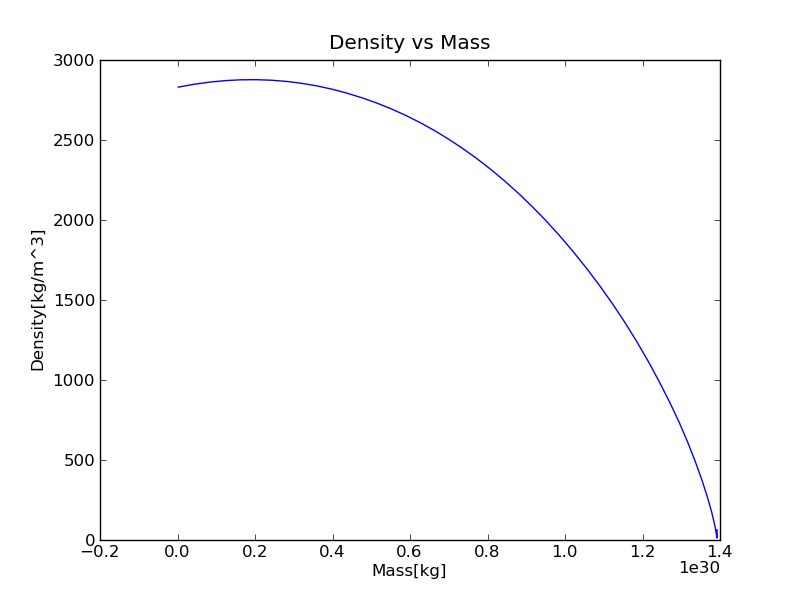
\includegraphics[width=\textwidth]{Calculate_density/Density_for_rho_p_t_others_constant}
      \caption{Using equation of state for density}
      \label{fig:Density_density}
    \end{subfigure}
    \begin{subfigure}{0.49\textwidth}
      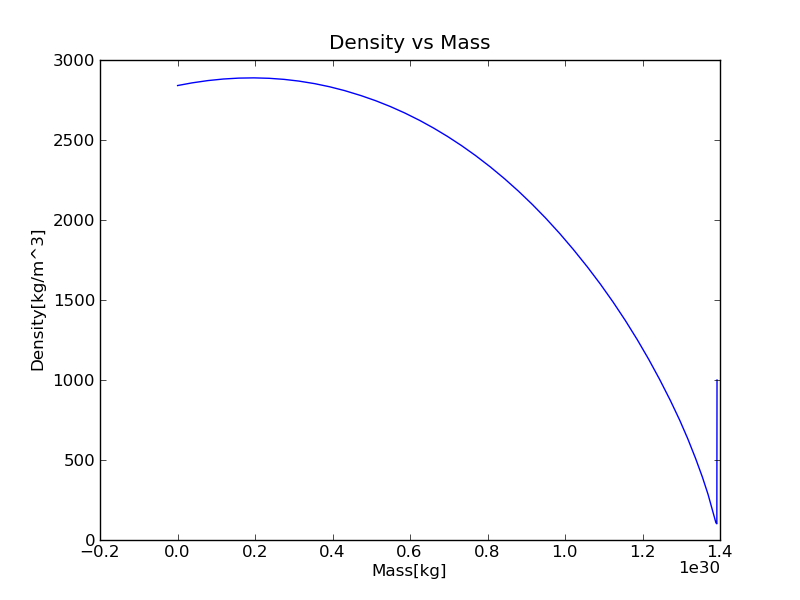
\includegraphics[width=\textwidth]{Calculate_pressure/Density_for_rho_p_t_others_constant}
      \caption{Using equation of state for pressure}
      \label{fig:Density_pressure}
      \end{subfigure}
\end{figure}

\begin{figure}[H]
    \centering
    \begin{subfigure}{0.49\textwidth}
      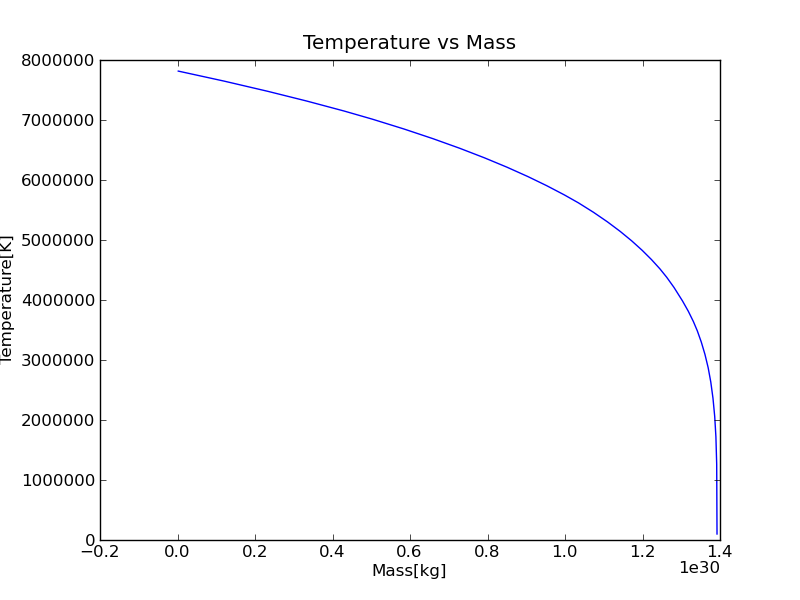
\includegraphics[width=\textwidth]{Calculate_density/Temperature_for_rho_p_t_others_constant}
      \caption{Using equation of state for density}
      \label{fig:Temp_density}
    \end{subfigure}
    \begin{subfigure}{0.49\textwidth}
      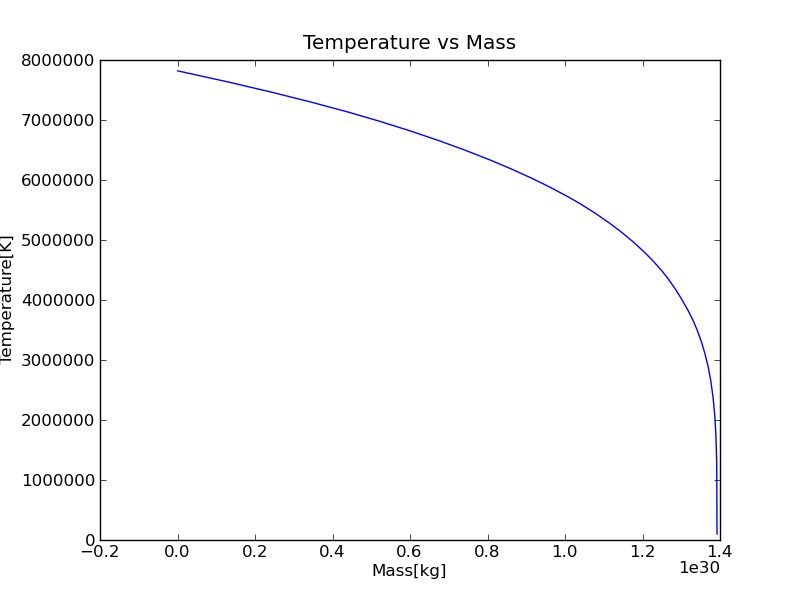
\includegraphics[width=\textwidth]{Calculate_pressure/Temperature_for_rho_p_t_others_constant}
      \caption{Using equation of state for pressure}
      \label{fig:Temp_pressure}
    \end{subfigure}
\end{figure}

\begin{figure}[H]
    \centering
    \begin{subfigure}{0.49\textwidth}
      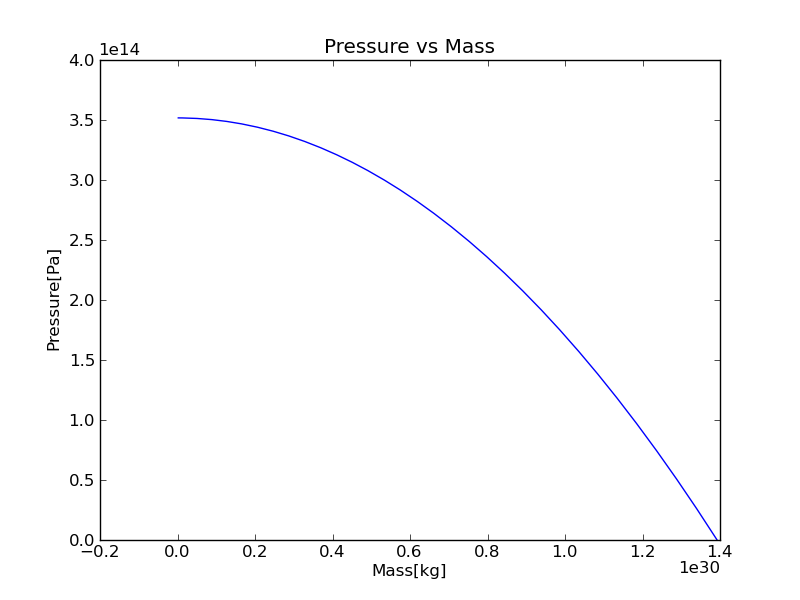
\includegraphics[width=\textwidth]{Calculate_density/Pressure_for_rho_p_t_others_constant}
      \caption{Using equation of state for density}
      \label{fig:Pressure_density}
    \end{subfigure}
    \begin{subfigure}{0.49\textwidth}
      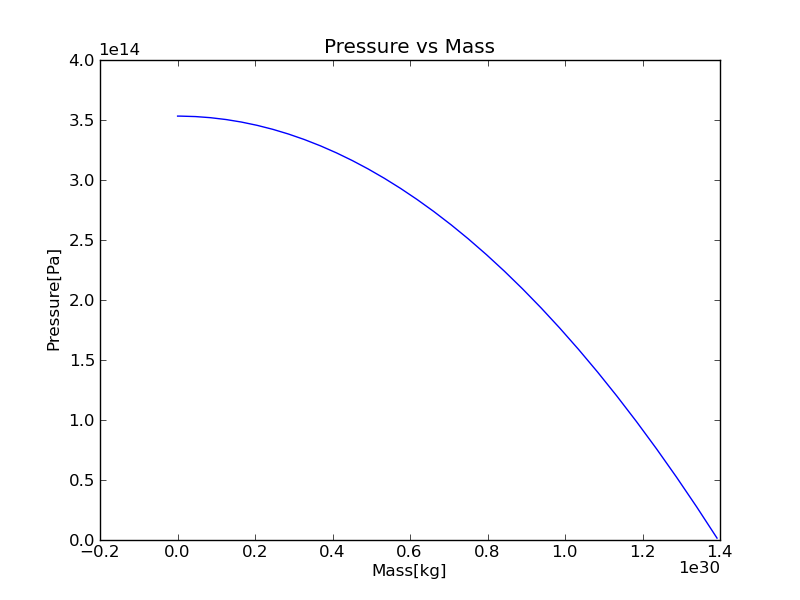
\includegraphics[width=\textwidth]{Calculate_pressure/Pressure_for_rho_p_t_others_constant}
      \caption{Using equation of state for pressure}
      \label{fig:Pressure_pressure}
    \end{subfigure}
\end{figure}



If we calculate the start pressure from the equation of state and look at the density we get a large change in the beginning and an end value of around 3000 Pa.
Doing the same, but instead calculating the density from the equation of state gives a smoother change in the beginning and an end value of about 3000 Pa.

If one now tries to change the start values of the variables not calculated by the equation of state, one gets varying degrees of "jumps" in the beginning. This happens when both multiplying and dividing $P_0$ by 10, and also when dividing $T_0$ by 2 or multiplying by 10. 

%Density
\begin{figure}[H]
    \centering
    \begin{subfigure}{0.49\textwidth}
      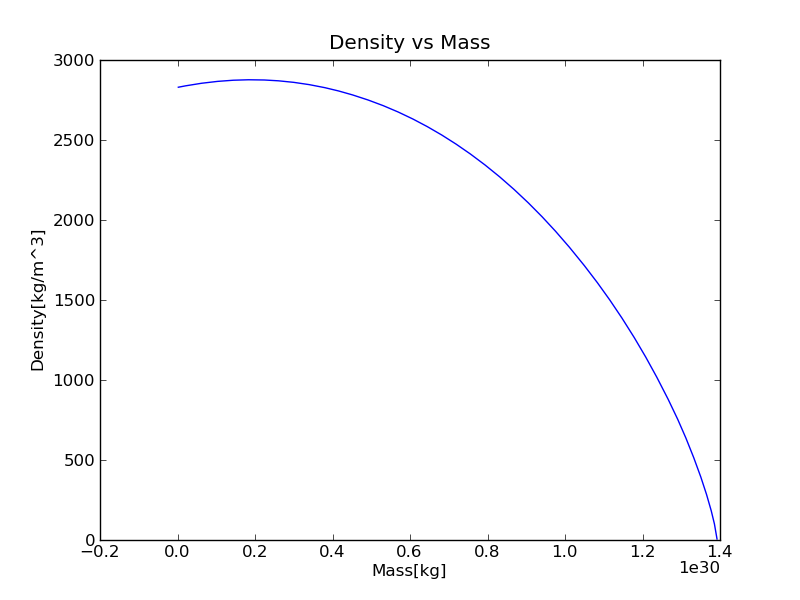
\includegraphics[width=\textwidth]{Calculate_density/Density_for_rho_p_t_others_constant_Pdiv10}
      \caption{Dividing $P_0$ by 10}
      \label{fig:density_denisity_Pdiv10}
    \end{subfigure}
    \begin{subfigure}{0.49\textwidth}
      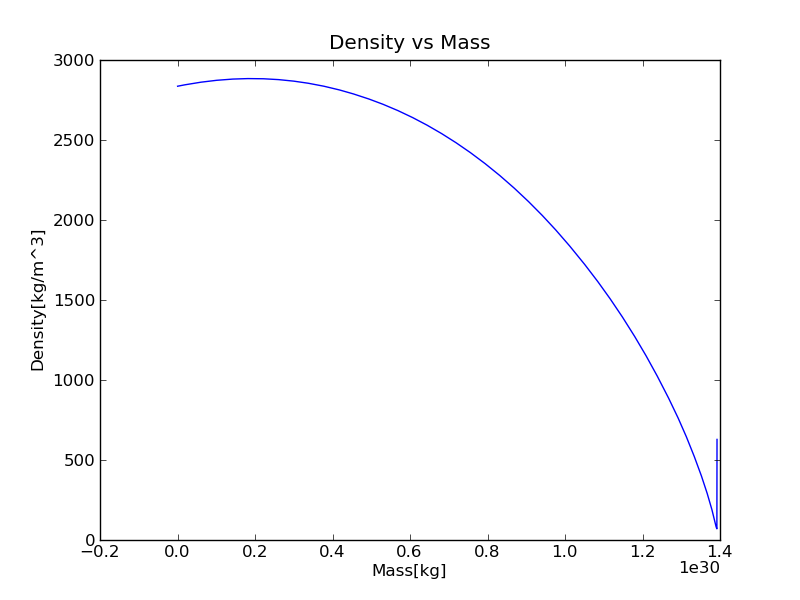
\includegraphics[width=\textwidth]{Calculate_density/Density_for_rho_p_t_others_constant_Ptimes10}
      \caption{Multiplying $P_0$ by 10}
      \label{fig:density_density_Ptimes10}
    \end{subfigure}
    \caption{Using the equation of state to calculate density}
\end{figure}
%Temperature
\begin{figure}[H]
    \centering
    \begin{subfigure}{0.49\textwidth}
      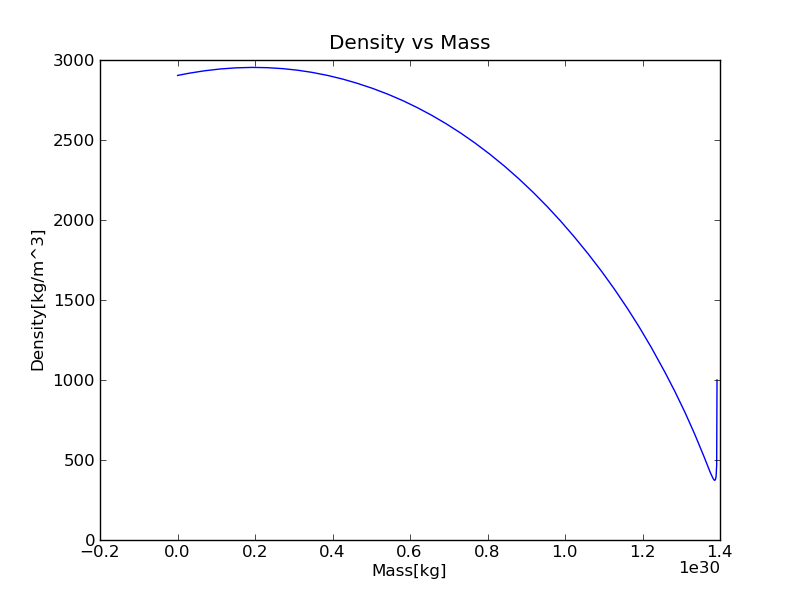
\includegraphics[width=\textwidth]{Calculate_pressure/Density_for_rho_p_t_others_constant_Ttimes0_6}
      \caption{Multiplying $T_0$ by 0.6}
      \label{fig:density_pressure_Ttimes0_6}
    \end{subfigure}
    \begin{subfigure}{0.49\textwidth}
      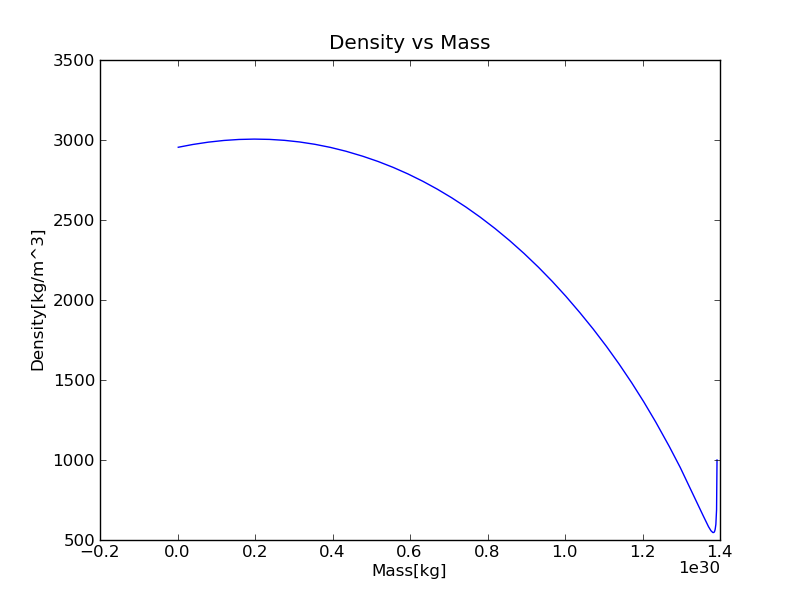
\includegraphics[width=\textwidth]{Calculate_pressure/Density_for_rho_p_t_others_constant_Ttimes10}
      \caption{Multiplying $T_0$ by 10}
      \label{fig:density_pressure_Ttimes10}
    \end{subfigure}
    \caption{Using the equation of state to calculate pressure}
\end{figure}

\begin{figure}[H]
    \centering
    \begin{subfigure}{0.49\textwidth}
      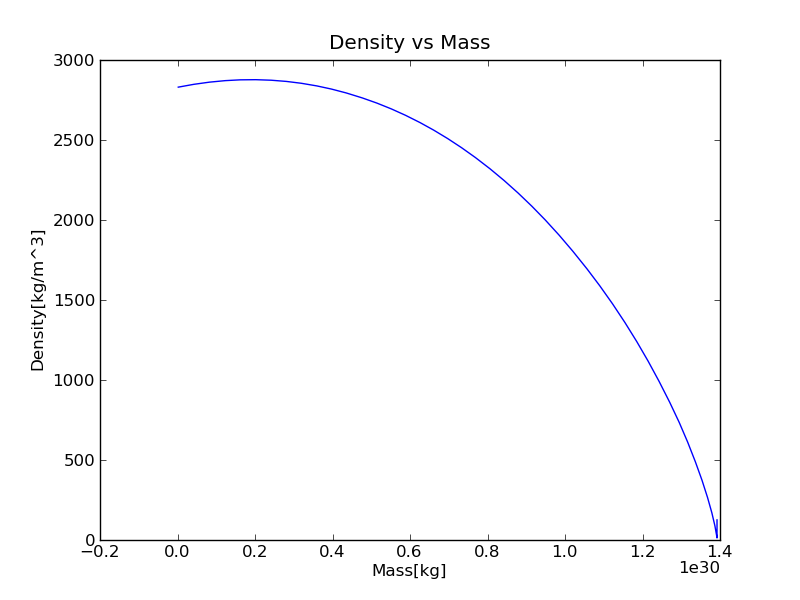
\includegraphics[width=\textwidth]{Calculate_density/Density_for_rho_p_t_others_constant_Tdiv2}
      \caption{Dividing $T_0$ by 2}
      \label{fig:density_density_Tdiv2}
    \end{subfigure}
    \begin{subfigure}{0.49\textwidth}
      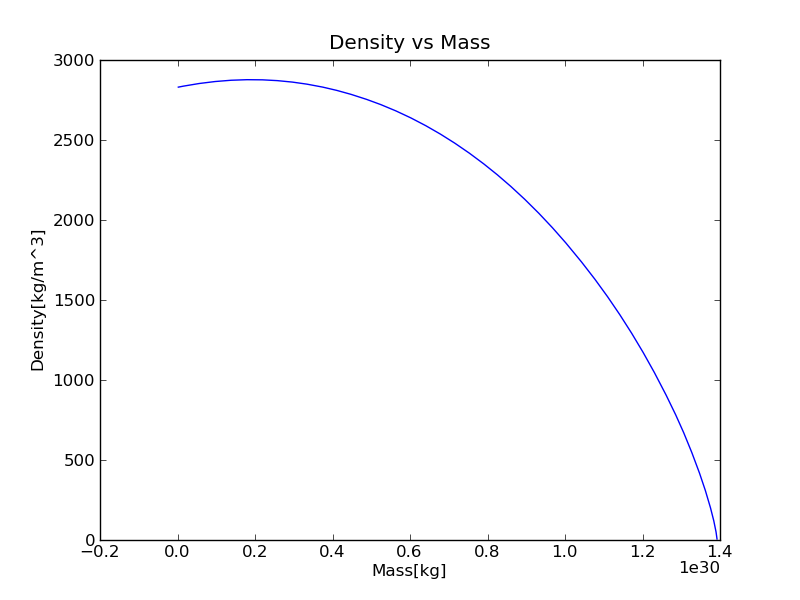
\includegraphics[width=\textwidth]{Calculate_density/Density_for_rho_p_t_others_constant_Ttimes10}
      \caption{Multiplying $T_0$ by 10}
      \label{fig:density_density_Ttimes10}
    \end{subfigure}
    \caption{Using the equation of state to calculate density}
\end{figure}



The same happens when varying $\rho_0$. However, if we go one step further and multiply $T_0$ by 100. We get a smooth start, and we don't get the decrease in density which all of the other variations had. This works when both calculating $P_0$ and $\rho_0$ from the equation of state. There is however one important difference; when calculating the pressure with the equation of state, the density stabilizes a little below 3000 Pa, while if you calculate density using the equation of state you get a density that stabilizes a little above 2000 Pa.

\begin{figure}[H]
    \centering
    \begin{subfigure}{0.49\textwidth}
      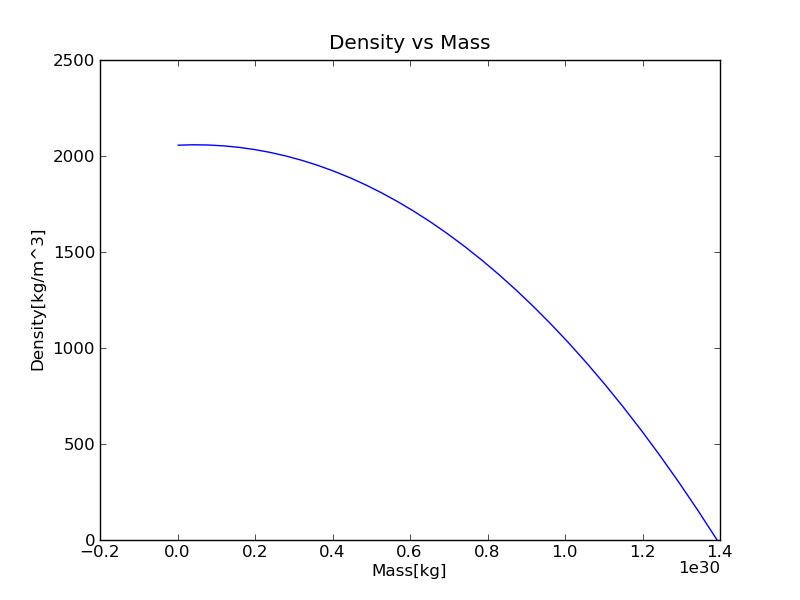
\includegraphics[width=\textwidth]{Calculate_density/Density_for_rho_p_t_others_constant_Ttimes100}
      \caption{Using the equation of state to calculate density}
      \label{fig:density_density_Ttimes100}
    \end{subfigure}
    \begin{subfigure}{0.49\textwidth}
      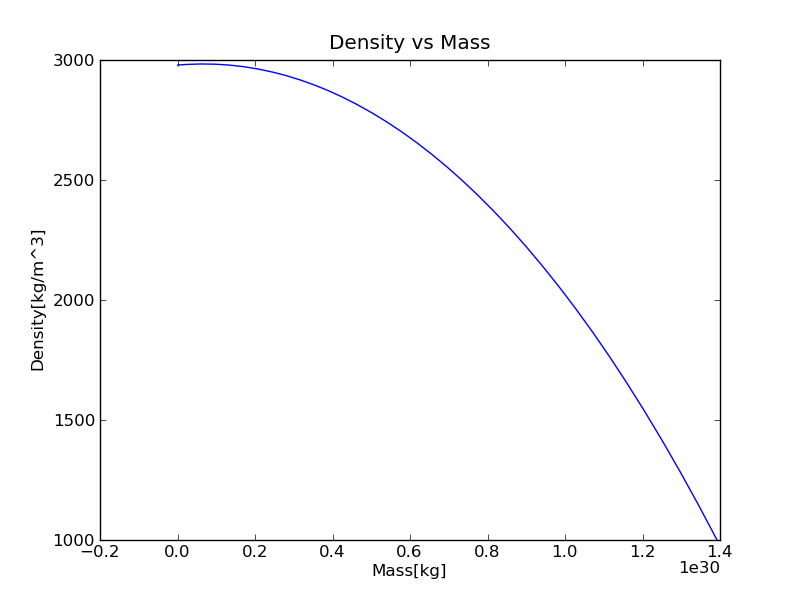
\includegraphics[width=\textwidth]{Calculate_pressure/Density_for_rho_p_t_others_constant_Ttimes100}
      \caption{Using the equation of state to calculate pressure}
      \label{fig:density_pressure_Ttimes100}
    \end{subfigure}
    \caption{Multiplying $T_0$ by 100 for both approaches}
\end{figure}


 

Thus we have two "solutions", that can be used at a later point.

Next, let's look at the pressure.The two reference plots look exactly the same. 
The same can also be said even if one changes $\rho_0$, $T_0$ and $P_0$ in the apropriate calculations. 
The plots hover around $3.5\times10^14 Pa$. 
The only exception is if one calculates the pressure with equation of state and then multiply $T_0$ by 10. 
This pushes the pressure up to about $3.75\times10^14 Pa$.

The temperature behaves in the same fashion. Whether we calculate pressure or density with the equation of state is irrelevant. It doesn't even change if we divide $\rho_0$ by 10, or multiply by 1.5. This is also the case if one multiplies $T_0$ by 0.6. Multiplying $T_0$ by 10 gives a smaller change in the beginning, but that's just because the start value is higher so there's not really anything special happening. The same thing happens when multipying $T_0$ by 100, making the change in temperature close to constant.
\begin{figure}[H]
    \centering
    \begin{subfigure}{0.49\textwidth}
      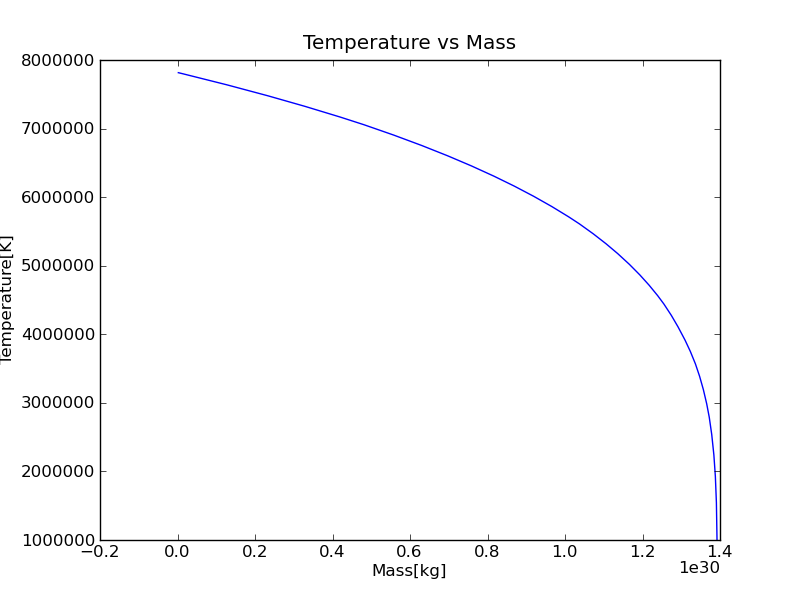
\includegraphics[width=\textwidth]{Calculate_density/Temperature_for_rho_p_t_others_constant_Ttimes10}
      \caption{Multiplying $T_0$ by 10}
      \label{fig:temperature_density_Ttimes10}
    \end{subfigure}
    \begin{subfigure}{0.49\textwidth}
      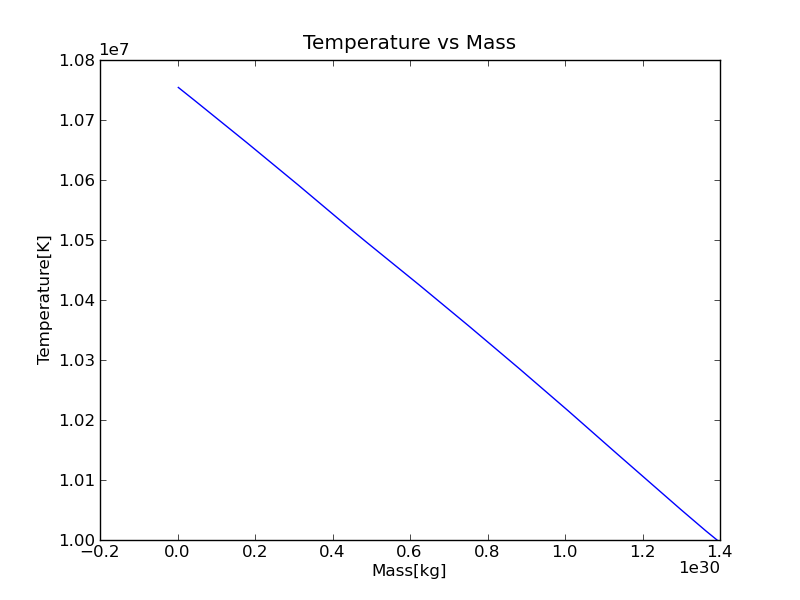
\includegraphics[width=\textwidth]{Calculate_density/Temperature_for_rho_p_t_others_constant_Ttimes100}
      \caption{Multiplying $T_0$ by 100}
      \label{fig:temperature_pressure_Ttimes100}
    \end{subfigure}
    \caption{Results for temperature equivalent for both approaches}
\end{figure}



From all of this testing we've found that we need a high temperature at the surface of the core if we want the density to behave in a reasonable manner.

\subsection{Getting R to go to zero, by changing $\rho_0$,$P_0$ and $T_0 $}
Now we want to get the radius to go to zero. To do this we need to find some density $rho_0$ that makes the radius go to zero before we run out of mass.
We want to be able to vary $\rho_0$ on our own.
At first glance, one may think that there are 4 ways to do this. However since we want to set $\rho_0$ by ourselves, we can't use the equation of state to find the density.
This leaves us with two ways. Both of them use the equation of state to find the pressure, but one sets the temperature constant, while the other sets the pressure constant.

First we try to set $P = 10^11$, and fix $T_0= 10^7$. Thus we can vary $\rho$ and find solution that seems best.
To start with we try running with $\rho_0 = 10^3$ as we've been doing from the start. This gives R values outside the opacity table. Increasing it doesn't help. 
Reducing it to $\rho_0 = 10^2$ works, but the mass is nowhere near zero. Reducing it further to $\rho_0 = 10$ gives approximately the same answer. 
The same happens for $\rho_0 = 10^-2$. And going lower gives R values outside the opacity table again. Clearly this is not the way to do this.

Instead we set $T = 10^7$, fix $P_0 = 10^11$, and then try some different values for $\rho_0$ that work.
This time we also start with $\rho_0 = 10^3$. This gives the same problem as earlier, but at least the mass is reduced a little. Next we reduce it to $\rho_0 = 10^2$. This makes the mass stay almost constant. Next we try increasing it to $\rho_0 = 10^4$, and now the mass goes to zero while the radius stays almost constant! Thus there should be a value somewhere in between that sends them both to zero at approximately the same time!

\begin{figure}
\centering
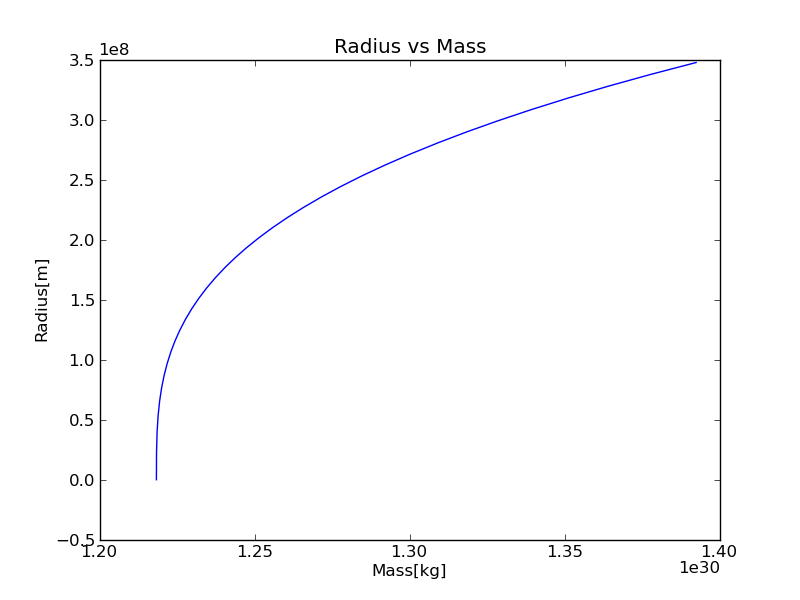
\includegraphics[width=\textwidth]{Radius_to_zero/fixP_rho1e3}
\caption{Radius goes to zero}\label{fig:radius_to_zero}
\end{figure}

This means that using this last approach is probably the best way to move forward with this model.

\subsection{Getting L,R and M to approach zero at the same time}
Now we want to get the luminosity, radius, and the mass to apporach zero at the same time.
At the time of writing this report I have not been able to accomplish this. I have been able to get the mass to apporach zero on its own. And I have also been able to get the luminosity to apporach zero on its own. I even found a range in $\rho_0$ that if $\rho_0$ was less than some number, one of them went to zero, while if $\rho_0$ was above it, the other one went to zero.

Thus the problem is getting the radius $r$ to approach zero. To accomplish this we want $dr$ to be as large as possible. And looking at the equation for $dr$, one can see that this is accomplished by having as small radius $r$ as possible and as small density $\rho$ as possible. I have tried setting  $\rho_0$ as small as $10^{-8}$ and $R_0$ as small as $0.1R_{\odot}$. This accomplishes nothing. 

I've also considered that the luminosity may be going to zero too fast. Looking at the equation for $dL$ one problem could be that the temperature is too high. However, if I try setting the temperature $T_0$ lower than about $10^4$ I get problems with values being outside the opacity table. Looking at the equation for $dL$ a second time reveals that we can also reduce $\rho_0$ to minimize it, but that's already been tried. I've also tried plotting the energy production as a function of temperature and when doing that you can clearly see that the lower the temperature is, the lower the energy production is. Thus there is no magic point at a higher temperature where it suddenly falls off. The same is also true for the density $\rho$.

Another problem could be that the temperature grows too fast. So if one looks at the equation for $dT$, one can see that we want as low luminosity $L_0$ as possible, and as high radius $R_0$ and temperature $T_0$ as possible. But all of these things have been tried, except for reducing the luminosity, but that would defeat the purpose of this whole model, since the luminosity must be at its maximum at the surface of the core. Thus the luminosity $L_0$ at the surface of the core must be the solar luminosity $L_\odot$.

At this point I'm out of ideas.

\newpage
\section{Appendix}
\subsection{The python code}
\begin{verbatim}
"""
Term Project 1
The first term project involves modeling the central parts of the sun by
writing a computer program to solve the governing equations. The project
involves information contained in Chaps.1-5.

The project can be found at 
http://www.uio.no/studier/emner/matnat/astro/AST3310/v15/notes/term1v1.pdf

Created by Andreas Ellewsen
"""
from numpy import exp,zeros,array_equal\
,genfromtxt,log10,pi    #Numerical python
from matplotlib.pyplot import plot,figure\
,title,xlabel,ylabel,show	#Plotting library
import sys as sys

#Constants
G	= 6.67384E-11		#[m**3*kg**-1*s**-2] Gravitational constant
m_u 	= 1.66053892173E-27 	#[kg] Atomic mass unit
N_A 	= 6.0221413E23      	#[] Avogadros number
k   	= 1.3806488E-23		#[m**2*kg*s**-2*K**-1] Boltzmans constant
c	= 2.99792458E8		#[m*s**-1] Speed of lights in vacuum
sigma   = 5.67E-8		#[W*m**-2*K**-4] Stefan-Boltzmans constant
MeVtoJ 	= 1.60217657E-13 	#[J] Conversion factor from MeV to Joules
L_sun  	= 3.846E26		#[W] Luminosity of the sun
R_sun  	= 6.958E8		#[m] Radius of the sun
M_sun  	= 1.989E30		#[kg] Mass of the sun

#Energy output of reactions
Q_pp = (.15+1.02)  *MeVtoJ	#[J]
Q_dp = (5.49)	   *MeVtoJ	#[J]
Q_33 = (12.86)	   *MeVtoJ	#[J]
Q_34 = (1.59)	   *MeVtoJ	#[J]
Q_7e = (.05)	   *MeVtoJ	#[J]
Q_71prime = (17.35)*MeVtoJ	#[J]

#Initial conditions
X       = .7        	#[] Hydrogen fraction
Y3      = 1E-10     	#[] Helium 3 fraction
Y       = .29	    	#[] Sum of Helium 3 and Helium 4 fractions
Y4      = Y-Y3      	#[] Helium 4 fraction
Z_73Li  = 1E-13      	#[] Lithium  fraction
Z_74Be  = 1E-13     	#[] Berylium fraction
Z       = .01		#[] Other
L_0     =  L_sun    	#[W] Luminosity of the star
R_0     = .5*R_sun   	#[m] Radius of the star
M_0     = .7*M_sun	#[kg] Mass of star 
rho_0   = 1e3		#[kg*m**-3] Mass density of star 
T_0     = 1E5	  	#[K] Temperature
#P_0     = 1E11		#[Pa] Pressure


#Computes number of atoms of the different elements.
def atomnumbers(rho):
	n_e   = rho*(1+X) /(2.*m_u)    	#Number of electrons
	n_d   = 0			#Number of deuterium atoms
	n_p   = rho*X	  /m_u     	#Number of Hydrogen atoms
	n_3   = rho*Y3	  /(3.*m_u)     #Number of Helium 3 atoms
	n_4   = rho*Y4	  /(4.*m_u)     #Number of Helium 4 atoms
	n_Li  = rho*Z_73Li/(7.*m_u) 	#Numver of Beryllium 7 atoms
	n_Be  = rho*Z_74Be/(7.*m_u) 	#Number of Lithium 7 atoms
	atomnumbers = [n_e,n_d,n_p,n_3,n_4,n_Li,n_Be]
	return atomnumbers

#Reactions
"""In this part the reaction rates of the processes in the PPI and PPII \
chain are calculated. I neglect the other processes since I choose to \
look at a star with low temperature at it's core, and in that case those \
processes are very slow compared to PPI and PPII."""

def reactions(T):
	T9 		= T*1E-9		#Convert T to form used in reactions.
	T9_star1 	= T9/(1+4.95E-2*T9)	#Other form used.
	T9_star2 	= T9/(1+.759*T9)	#Yet another form used.

	H_D   	= 	4.01E-15*T9**(-2./3)*exp(-3.380*T9**(-1./3))*(1 +\
                     .123*T9**(1./3) + 1.09*T9**(2./3) + .938*T9)

	He3_p	= 	6.04E10*T9**(-2./3)*exp(-12.276*T9**(-1./3))*(1 +\
                     .034*T9**(1./3) - .522*T9**(2./3)-.124*T9 + \
                     .353*T9**(4./3)+ .213*T9**(-5./3))

	He3_Be  = 	5.61E6*T9_star1**(5./6)*T9**(-3./2)*exp(-12.826*\
                     T9_star1**(-1./3))

	Be_Li   = 	1.34E-10*T9**(-1./2)*(1 - .537*T9**(1./3)  + \
                     3.86*T9**(2./3) +  .0027*T9**-1*exp(2.515E-3*T9**-1))

	Li_p	= 	     1.096E9*T9**(-2./3)*exp(-8.472*T9**(-1./3)) - \
                     4.830E8*T9_star2**(5./6)*T9**(-3./2)*exp(-8.472*\
                     T9_star2**(-1./3)) + 1.06E10*T9**(-3./2)\
                     *exp(-30.442*T9**-1)
	"""
	"These two reactions are not used in this assignment, but may be useful \
     at a later point, so I've kept them here."
     
	Berylliym_Boron = 	3.11E5*T9**(-2./3)*exp(-10.262*T9**(-1./3))+2.53E3\
                         *T9**(-3./2)*exp(-7.306*T9**-1)

	Nitrogen_Oxygen = 	4.9E7*T9**(-2./3)*exp(-15.228*T9**(-1./3)-\
                         .092*T9**2)*(1+.027*T9**(1./3)-.778*T9**(2./3)\
                         -.149*T9+.261*T9**(4./3)+.127*T9**(5./3)) + \
                         2.37E3*T9**(2./3)*exp(-3.011*T9**-1) + \
                         2.19E4*exp(-12.53*T9**-1)
	"""
	rrs = [H_D,He3_p,He3_Be,Be_Li,Li_p]#,Berylliym_Boron,Nitrogen_Oxygen
	return rrs

#Time evolution
"""This segement takes care of the time evolution of the reactions. 
By doing this we hope to reach some kind of equilibrium over time, 
such that all the reaction rates stabilize at some level. 
This is achieved remarkably fast, as can be seen in the choice of Time 
and steps N."""
def Reactionrates(T,rho):
	counter = 0
	Time  = 1		#Total time to simulate [s]
	N  = 10**4		#Number of steps
	dt = Time/N		#Timesteps [s]
	n = atomnumbers(rho)
	rrs = reactions(T)
	reactionrate_old = zeros(6)
	reactionrate_new = zeros(6)
	for i in range(0,N-1):
		#Reaction rates
		"""All of the following rates are calculated by the equation
		r_ik = n_i*n_k/(rho*(1+delta_ik)*lambda_ik)
		where i,k define the elements and delta_ik =1 if i=k else 0.
		"""
		lambda_pp = rrs[0]/N_A*1E-6		#[m^3/s]
		lambda_pd = 1				#This one is actually unknown so it's just \
							#set to 1 since the reaction it is used in 
							#includes the number of deuterium atoms and \
							#that number is set to 0 earlier.
		lambda_33 = rrs[1]/N_A*1E-6		#[m^3/s]
		lambda_34 = rrs[2]/N_A*1E-6		#[m^3/s]
		lambda_7e = rrs[3]/N_A*1E-6		#[m^3/s]
		lambda_71prime  = rrs[4]/N_A*1E-6	#[m^3/s]
		#lambda_71  = Berylliym_Boron/N_A*1E-6	#[m^3/s]#Not used in this assigment
		#lambda_p14 = Nitrogen_Oxygen/N_A*1E-6	#[m^3/s]#Not used in this assigment

		r_pp 	  = n[2]**2/(rho*2)*lambda_pp	#[kg-1*s-1]
		r_pd  	  = r_pp			#[kg-1*s-1] Assume this reaction happens \
							#instantly such that it happens at the same \
							#rate as the elements it needs become available.
							#Thus it must be the same as the reaction that \
							#creates those elements (in this case Deuterium)
		r_33 	  = n[3]**2  /(rho*2)*lambda_33	#[kg-1*s-1]
		r_34 	  = n[3]*n[4]/rho*lambda_34	#[kg-1*s-1]
		r_7e 	  = n[5]*n[6]/rho*lambda_7e	#[kg-1*s-1]
		r_71prime = n[5]*n[2]/rho*lambda_71prime#[kg-1*s-1]
		#r_71  	 = n_Li*n_p	/rho*lambda_71	#Not used in this assigment
		#r_p14 	 = n_p*n_4	/rho*lambda_p14 #Not used in this assigment
		
		#This part makes sure that reaction rates which rely on other rates \
		#don't use elements that are not yet present.
		if (2./3)*r_33 + (1./3)*r_34 > r_pp:
			r_34 = (1./3)*r_pp
			r_33 = (2./3)*r_pp
		if r_7e > r_34:
			r_7e = r_34
		if r_71prime > r_7e:
			r_71prime = r_7e
		reactionrate_new = r_pp,r_pd,r_33,r_34,r_7e,r_71prime
		#print 'round:',i

		if array_equal(reactionrate_old,reactionrate_new) == True:
			counter +=1
		if counter == 20:
			counter = 0
			break
		reactionrate_old = reactionrate_new

		#Evolution of element abundances

		"""This part updates the number of Hydrogen atoms and Helium 4 atoms.
		We choose to neglect updating the rest of the elements since there \
		are so few of them, and thus their contribution is small."""
		d_npdt   = -n[2]**2.*lambda_pp 	- n[1]*n[2]*lambda_pd + n[3]**2.*\
			   lambda_33 - n[5]*n[2]*lambda_71prime
		d_nHe4dt = (n[3]**2.)/2.*lambda_33 - n[3]*n[4]*lambda_34 + 2.*n[5]\
			   *n[2]*lambda_71prime 
		n[2] 	+= dt*d_npdt 	    	#Number of Hydrogen atoms
		n[4] 	+= dt*d_nHe4dt   	#Number of Helium 4 atoms
	return reactionrate_new

#Solving the equation for the change in Luminosity

def Energy(T,rho):
	reactionrate = Reactionrates(T,rho)
	e_1  = reactionrate[0]*(Q_pp+Q_dp)
	e_2  = reactionrate[2]*Q_33
	e_3  = reactionrate[3]*Q_34
	e_4  = reactionrate[4]*Q_7e
	e_5  = reactionrate[5]*Q_71prime
	e    = e_1+e_2+e_3+e_4+e_5
	return e

#Defining functions for pressure,temperature and density
"""This part solves the equation for Pressure, assuming 
the equation of state to be that of an ideal gas"""

#Constants needed
mu 	= 1/(2.*X + 7./4*Y + 5./7*Z_74Be + 4./7*Z_73Li + 9./16*Z)
a 	= 4.*sigma/c

def Pressure(rho,T):
	#P_rad 	= a/.3*T**4		#Radiation pressure
	P_G 	= rho*k*T/(mu*m_u)    	#Gas pressure, assuming ideal gas
	P	= P_G #+ P_rad 		#Total Pressure
	return P

def Density(P,T):
	rho  = (P*mu*m_u)/(k*T)		#Ideal gas
	#rho = (m_u*mu)/(k*T)*(P - (a*T**4)/3.)	#Includes radiation pressure
	return rho

def Temperature(rho,P):
	T = (P*mu*m_u)/(k*rho)
	return T

"""
#Start of test area for Energy Production
#Test with core of the sun
rho     = 1.62E5    #Mass density of star [kg*m**-3]
T       = 1.57E7    #Temperature    [K]
X       = .7        #Hydrogen fraction
Y3      = 1E-10     #Helium 3 fraction
Y 	= .29 	    #Sum of Helium 3 and Helium 4 fractions
Y4      = Y-Y3      #Helium 4 fraction
Z_73Li  = 1E-7      #Lithium  fraction
Z_74Be  = 1E-7      #Berylium fraction
T   	= 1.57E7
rho 	= 1.62E5
reactionrate = Reactionrates(T,rho)
print "%.2e"%(reactionrate[0]*(Q_pp + Q_dp)*rho)
print "%.2e"%(reactionrate[2]*Q_33*rho)
print "%.2e"%(reactionrate[3]*Q_34*rho)
print "%.2e"%(reactionrate[4]*Q_7e*rho)
print "%.2e"%(reactionrate[5]*Q_71prime*rho)

dLdm = Energy(T_0,rho_0)
print "dL/dm = %.2e"%dLdm

P_0 = Pressure(rho_0,T_0)
print "P_0 = %.2e"%P_0
#End of test area for Energy Production
"""

#Function that reads the opacity table
lines = genfromtxt('opacity.txt')

def Opacity(T,rho):
	'''This function reads the opacity table'''
	#Convert R and T to the form used in opacity.txt
	R      = (rho*1E-3)/(T/1E6) 

	Rvalue = log10(R)
	Tvalue = log10(T)
	Rvalue = (round(2*Rvalue)/2.)
	if Rvalue >= 1.5 or Rvalue <= -8.5:
		print 'Tried using R outside opacity table'
		sys.exit()
	if Tvalue >= 8.8 or Tvalue <= 3.7 :
		print 'Tried using T outside opacity table'
		sys.exit()

	#Pick the right R value from the table
	for i in range(len(lines[0])):
		if Rvalue == lines[0][i]:
			Ri = i

   	#Make list of T values found in table
	Tlist = zeros(len(lines))
	for i in range(1,len(lines)):
		Tlist[i] = lines[i][0]

	#Pick the right T value from the table
	Ti = min(range(len(Tlist)), key=lambda i: abs(Tlist[i]-Tvalue))

	#Pick the right kappa value with R and T
	log10kappa = lines[Ti][Ri]

	#Convert the value given to the form used in the equations
	kappa = (10.**(log10kappa/10.))	
	return kappa


#Solving the five equations
'''This part solves all the five equations'''

#Make empty lists
R = []
L = []
P = []
T = []
M = []
rho = []
epsilon = []

#Fill the arrays with the initial conditions
M.append(M_0)
R.append(R_0)
L.append(L_0)
T.append(T_0)
rho.append(rho_0)
#P.append(P_0)
P.append(Pressure(rho[0],T[0]))
#rho.append(Density(P[0],T[0]))
#T.append(Temperature(rho[0],P[0]))
epsilon.append(Energy(T[0],rho[0]))


#Simulate evolution by reducing mass.
i = 0     #Starts the counter
p = 0.01 #Max change allowed

while M[i] > 0 and R[i] > 0 and L[i] > 0 and T[i] > 0 and P[i] > 0:

    #Change in radius
    drdm 	= 1./(4*pi*R[i]**2*rho[i])
    dmr 	= p*R[i]/drdm    

    #change in Pressure
    dPdm 	= -(G*M[i])/(4*pi*R[i]**4)
    dmP 	= p*P[i]/dPdm        

    #Change in Luminosty
    dLdm 	= epsilon[i]		
    dmL 	= p*L[i]/dLdm    

    #Change in temperature
    kappa   	= Opacity(T[i],rho[i])		#Opacity
    dTdm    	= -3*kappa*L[i]/(256*pi**2*sigma*R[i]**4*T[i]**3)
    dmT 	= p*T[i]/dTdm

    #Change in density
    drhodm    	= (mu*m_u)/(k*T[i])*dPdm - (P[i]*mu*m_u)/(k*T[i]**2)*dTdm
    dmrho	= p*rho[i]/drhodm

    #Decide how small dm needs to be
    dmM =   10*p*M[i]
    dm  =   -min(abs(dmr),abs(dmP),abs(dmL),abs(dmT),abs(dmrho),abs(dmM))
    if abs(dm) < 1E3:
        dm = -1E3
    #Update values
    rho.append(rho[i] + drhodm*dm)
    M.append(M[i] + dm)			#Update mass
    R.append(R[i] + drdm*dm)		#Update Radius
    L.append(L[i] + dLdm*dm) 		#Update Luminosity
    P.append(P[i] + dPdm*dm)		#Update Pressure
    T.append(T[i] + dTdm*dm)		#Update Temperature
    epsilon.append(Energy(T[i],rho[i])) #Update energy output
    
    print 'M = %.3e, R = %.3e, L = %.3e, P = %.3e, T= %.3e, rho = %.3e, \
kappa = %.3e, epsilon = %.3e, dT = %.3e, dr = %.3e, dL = %.3e, dm = %.3e, \
dP = %.3e, drho = %.3e'%(M[i], R[i], L[i], P[i], T[i], rho[i], kappa, \
epsilon[i], dTdm*dm, drdm*dm, dLdm*dm, dm, dPdm*dm, drhodm*dm)


    i +=1   #increase counter

    #Print  information about which variable went to zero first.   
    if M[i] < 0:
        print 'Mass went negative'
	break
    if R[i] < 0:
        print 'Radius went negative'
	break
    if L[i] < 0:
        print 'Limuniosity went negative'
	break
    if T[i] < 0:
        print 'Temperature went negative'
	break
    if P[i] < 0:
        print 'Pressure went negative'
	break
  


#Scale values after initial conditions
"""for i in range(1,len(M)):
    M[i] = M[i]/M[0]
    
for i in range(1,len(R)):
    R[i] = R[i]/R[0]
    
for i in range(1,len(L)):
    L[i] = L[i]/L[0]
    
for i in range(1,len(P)):
    P[i] = P[i]/P[0]
    
for i in range(1,len(T)):
    T[i] = T[i]/T[0]
"""
#Plots of interesting things

figure()
plot(M,R)
title('Radius vs Mass')
xlabel('Mass[kg]')
ylabel('Radius[m]')

figure()
plot(M,P)
title('Pressure vs Mass')
xlabel('Mass[kg]')
ylabel('Pressure[Pa]')

figure()
plot(M,L)
title('Luminosity vs Mass')
xlabel('Mass[kg]')
ylabel('Luminosity[W]')

figure()
plot(M,T)
title('Temperature vs Mass')
xlabel('Mass[kg]')
ylabel('Temperature[K]')

figure()
plot(M,rho)
title('Density vs Mass')
xlabel('Mass[kg]')
ylabel('Density[kg/m^3]')

figure()
plot(M,epsilon)
title('Energyproduction vs Mass')
xlabel('Mass[kg]')
ylabel('Energy[J/kg]')

show()
\end{verbatim}
\end{document}

